% !TEX encoding = UTF-8
% !TEX program = pdflatex
% !TEX root = presentazione.tex
% !TeX spellcheck = it_IT
%
\begin{frame}[t]{Tariffe - Confronti (3)}
	\begin{figure}[h]
	\centering
	    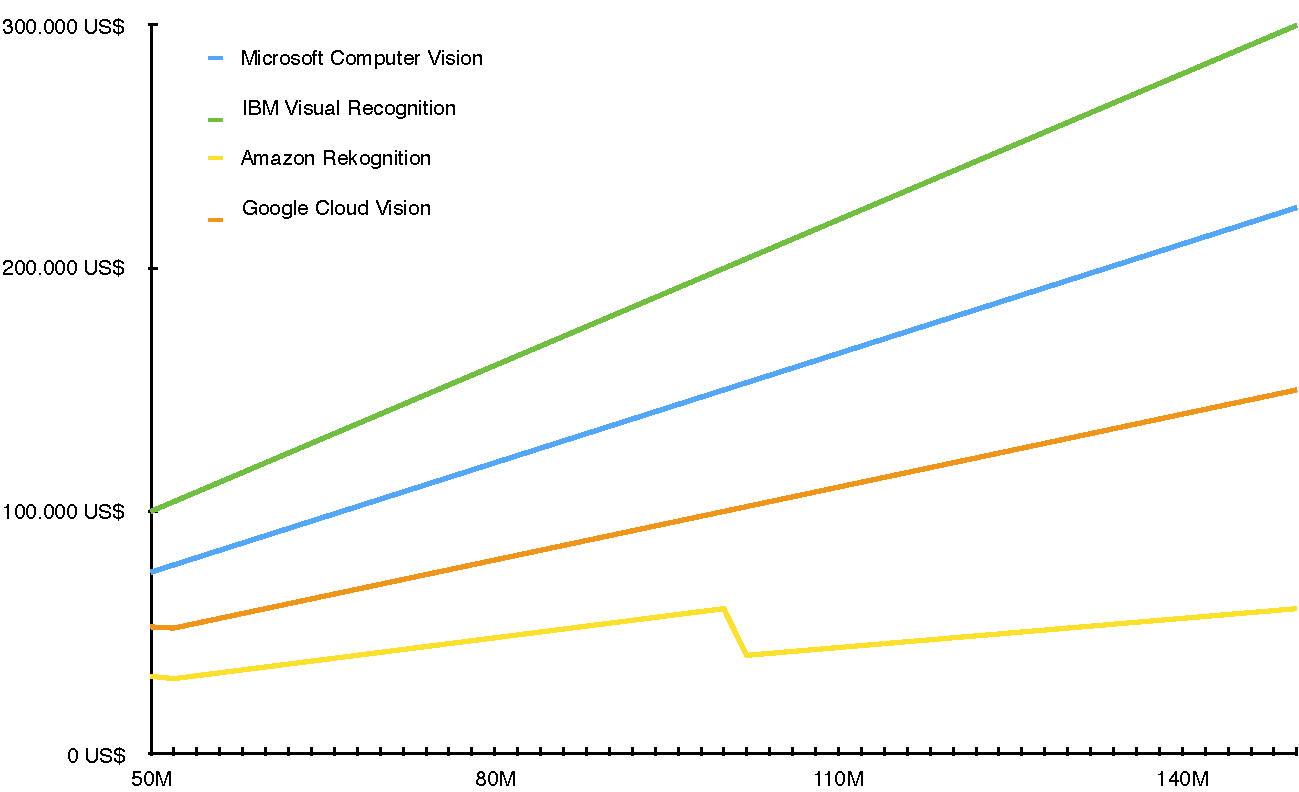
\includegraphics[width=.6\paperwidth,keepaspectratio=true]{../../doc/img/grafico3}
		{\tiny \caption{Riconoscimento oggetti (da 50M a 150M di immagini).}}
		\label{fig:tariffe-riconoscimento-oggetti-50-150M}
	\end{figure}
\end{frame}
%
%----------------------------------------------------------------------------------------
%	APPUNTI:
% 		- i prezzi sono proiezioni lineari di quelli base disponibili
%			per carichi così elevati probabilmente i prezzi si abbassano
%			- anche perché molti rendono disponibili prezzi fino a 20M altri fino a 1M
%		- TODO: sistemare: prima dicevo a chiamata, adessso uso a immagine.
%----------------------------------------------------------------------------------------
